% !TEX program = xelatex
% !TEX encoding = UTF-8 Unicode
% !BIB program = bibtex
% !TEX spellcheck = en_US
\documentclass[12pt]{article}
\usepackage[english]{babel}
\usepackage{url}
\usepackage{amsmath}
\usepackage{graphicx}
\usepackage{subfigure}
\graphicspath{{images/}}
\usepackage{parskip}
\usepackage{fancyhdr}
\usepackage{vmargin}
\usepackage{enumerate}
\usepackage[T1]{fontenc}
\usepackage{newpxtext,newpxmath}
\usepackage{booktabs}
\usepackage{siunitx}
\usepackage[version=4]{mhchem}
\usepackage{hyperref}
\usepackage{bm}
\usepackage{breqn}
\usepackage{miller}
\usepackage{braket}
\usepackage[space]{grffile}   % include graphics with spaces in their path


\setmarginsrb{1 cm}{2.5 cm}{1 cm}{2.5 cm}{1 cm}{1.5 cm}{1 cm}{1.5 cm}
\sisetup{inter-unit-product = \ensuremath{{}\cdot{}}}
\DeclareTextCommand{\nobreakspace}{T1}{\leavevmode\nobreak\ }

\title{Solid State Physics HW 7} % Title
\author{XYZ} % Author
\date{} % Date

\makeatletter
\let\thetitle\@title
\let\theauthor\@author
\let\thedate\@date
\makeatother

\pagestyle{fancy}
\fancyhf{}
\rhead{\theauthor}
\lhead{\thetitle}
\cfoot{\thepage}

\newcommand*{\rmn}[1]{\romannumeral#1}
\newcommand*{\RMN}[1]{\uppercase\expandafter{\romannumeral#1}}
 \newenvironment{mpmatrix}{\begin{medsize}\begin{pmatrix}}%
                {\end{pmatrix}\end{medsize}}%
\newcount\colveccount
\newcommand*\colvec[1]{
    \global\colveccount#1
    \begin{pmatrix}
        \colvecnext
    }
    \def\colvecnext#1{
        #1
        \global\advance\colveccount-1
        \ifnum\colveccount>0
        \\
        \expandafter\colvecnext
        \else
    \end{pmatrix}
    \fi
}
\newcommand*{\tran}{^{\mkern-1.5mu\mathsf{T}}}

\begin{document}

%%%%%%%%%%%%%%%%%%%%%%%%%%%%%%%%%%%%%%%%%%%%%%%%%%%%%%%%%%%%%%%%%%%%%%%%%%%%%%%%%%%%%%%%%

\begin{titlepage}
    \centering
    \vspace*{0.5 cm}
    
\includegraphics[scale = 0.25]{NewEngineeringDkBlue.png}\\[1.0 cm] % University Logo
    \textsc{\Large Applied Physics and Applied Mathematics\\
        \large with Materials Science and Engineering}\\[2.0 cm] % University Name
    \textsc{\Large APPH 6081}\\[0.5 cm]    % Course Code
    \rule{\linewidth}{0.2 mm} \\[0.4 cm]
    { \huge \bfseries \thetitle}\\
    \rule{\linewidth}{0.2 mm} \\[1.5 cm]

    \begin{minipage}{0.4\textwidth}
        \begin{flushleft} \large
            \emph{Submitted To:}\\
            Chris Marianetti\\
            Assoc. Professor\\
            APAM Department\\
        \end{flushleft}
    \end{minipage}~
    \begin{minipage}{0.4\textwidth}

        \begin{flushright} \large
            \emph{Submitted By :} \\
            XYZ\\
            \texttt{xyz}\\
            Fall 2016\\
        \end{flushright}

    \end{minipage}\\[2 cm]
\end{titlepage}

\section{Problem \RMN{1}}
\begin{enumerate}[(a)]
    \item  From last homework, we derive the total Hamiltonian under the orbital
          basis, written as
          \begin{equation}
              \begin{split}
                  H_{\bm{k}}
                   & = \begin{pmatrix}
                           \varepsilon_d & t_{pd}        \\
                           t_{pd}        & \varepsilon_p \\
                       \end{pmatrix} + \exp(ika)
                  \begin{pmatrix}
                      0      & 0 \\
                      t_{pd} & 0 \\
                  \end{pmatrix} +
                  \exp(-ika)
                  \begin{pmatrix}
                      0 & t_{pd} \\
                      0 & 0      \\
                  \end{pmatrix}                                  \\
                   & = \begin{pmatrix}
                           \varepsilon_p + 1   & t_{pd}(1+\exp(-ika)) \\
                           t_{pd}(1+\exp(ika)) & \varepsilon_p        \\
                       \end{pmatrix}.
              \end{split}
          \end{equation}
          So the eigenvalues of the Hamiltonian is
          \begin{equation}\label{eq:1d}
              \varepsilon(k)=\varepsilon_p + \frac{1}{2} \pm \frac{1}{2}\sqrt{\cos^2\frac{k a}{2}+1}.
          \end{equation}
          Select $\varepsilon_p = \frac{1}{2}$, then
          see Fig. \ref{fig:1-a} for the band structure plot of the result in the first BZ.
          \begin{figure}[h]
              \centering
              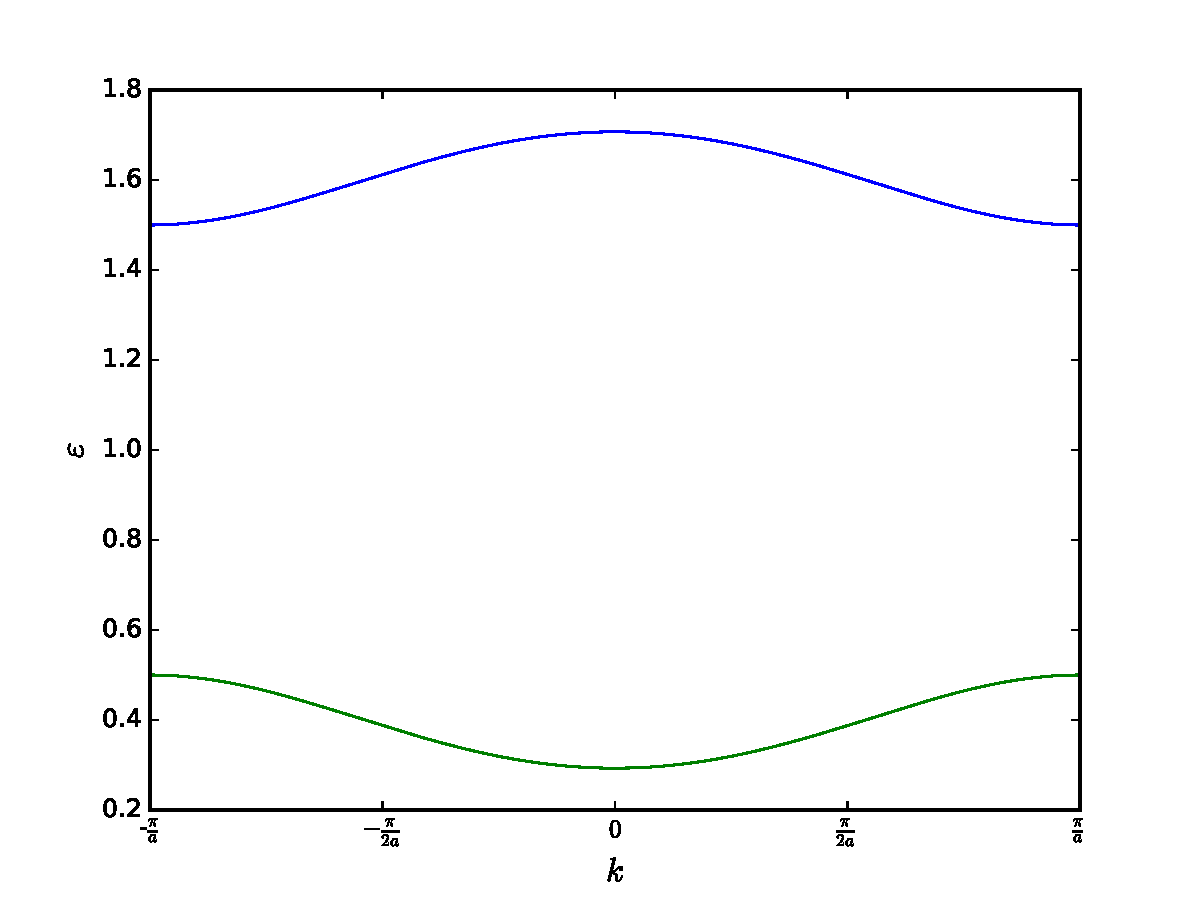
\includegraphics[width=0.7\linewidth]{pro_1_a.pdf}
              \caption{Band structure plot of the result in the first BZ.}
              \label{fig:1-a}
          \end{figure}
    \item Derive $\nabla_{\bm{k}} \varepsilon(\bm{k})$ we have
          \begin{equation}
              \begin{split}
                  \nabla_{\bm{k}} \varepsilon(\bm{k})
                   & = \pm\frac{2 a t^2 \sin (a k)}{\sqrt{8 t^2 (\cos (a k)+1)+1}}                                                                                                                  \\
                   & = \pm\frac{a \sqrt{(4 (\varepsilon -\varepsilon_p +\frac{1}{2})^2-1) (-4 (\varepsilon -\varepsilon_p +\frac{1}{2})^2+16 t^2+1)}}{8 (\varepsilon -\varepsilon_p +\frac{1}{2})},
              \end{split}
          \end{equation}
          if we let $\varepsilon_p - \frac{1}{2} = 0$, then
          \begin{equation}
              \nabla_{\bm{k}} \varepsilon(\bm{k}) =
              \pm\frac{a \sqrt{(4 \varepsilon^2-1) (-4 \varepsilon^2+16 t^2+1)}}{8 \varepsilon}.
          \end{equation}
          so the DOS is
          \begin{equation}
              \begin{split}
                  g(\varepsilon)
                   & = \frac{1}{\pi}
                  \int_{S_n(\varepsilon)} dS\frac{1}{\Big\lvert \frac{a \sqrt{(4 \varepsilon^2-1) (-4 \varepsilon^2+16 t^2+1)}}{8 \varepsilon} \Big\rvert} \\
                   & = \frac{1}{\pi}
                  \int_{S_n(\varepsilon)} dS
                  \bigg\lvert\frac{8 \varepsilon}{a \sqrt{(4 \varepsilon^2-1) (-4 \varepsilon^2+16 t^2+1)}}\bigg\rvert                                     \\
                   & = \frac{16 \varepsilon}{a \sqrt{(4 \varepsilon^2-1) (-4 \varepsilon^2+16 t^2+1)}}
              \end{split}
          \end{equation}
          Or we have
          \begin{equation}
              N(\varepsilon) = \frac{2}{V_{\text{FBZ}}} \int dk \theta(\varepsilon
              -\varepsilon(k)),
          \end{equation}
          where $V_{\text{FBZ}} = \frac{2\pi}{a}$, $\varepsilon(k)$ is given by \eqref{eq:1d}.
          So
          \begin{equation}
              \begin{split}
                  N(\varepsilon) & = \frac{2}{\frac{2\pi}{a}} \int dk \theta(\varepsilon
                  -\varepsilon_p-\frac{1}{2}\pm \frac{1}{2}\sqrt{\cos^2\frac{k a}{2}+1)}                                                            \\
                                 & =  \frac{a}{\pi} k \bigg|_{-\frac{1}{a}\arccos(8(\varepsilon-1)^2-3)}^{\frac{1}{a}\arccos(8(\varepsilon-1)^2-3)} \\
                                 & = \frac{2}{\pi}\arccos(8(\varepsilon-1)^2-3).
              \end{split}
          \end{equation}
          So the DOS is the derivative of $N(\varepsilon)$, written as
          \begin{equation}
              \begin{split}
                  g(\varepsilon) & = \frac{dN}{d\varepsilon}                                                         \\
                                 & = -\frac{32 (\varepsilon-1)}{\pi  \sqrt{1-\left(8 (\varepsilon-1)^2-3\right)^2}}.
              \end{split}
          \end{equation}
          Here $\varepsilon$ ranges from $0.292893$ to $0.5$, for $\varepsilon$ ranges from $1.5$ to $1.70711$,
          the density of states is
          \begin{equation}
              \begin{split}
                  g(\varepsilon) & = \frac{dN}{d\varepsilon}                                                        \\
                                 & = \frac{32 (\varepsilon-1)}{\pi  \sqrt{1-\left(8 (\varepsilon-1)^2-3\right)^2}}.
              \end{split}
          \end{equation}
          So plot as Fig. \ref{fig:pro1b}.
          \begin{figure}[h]
              \centering
              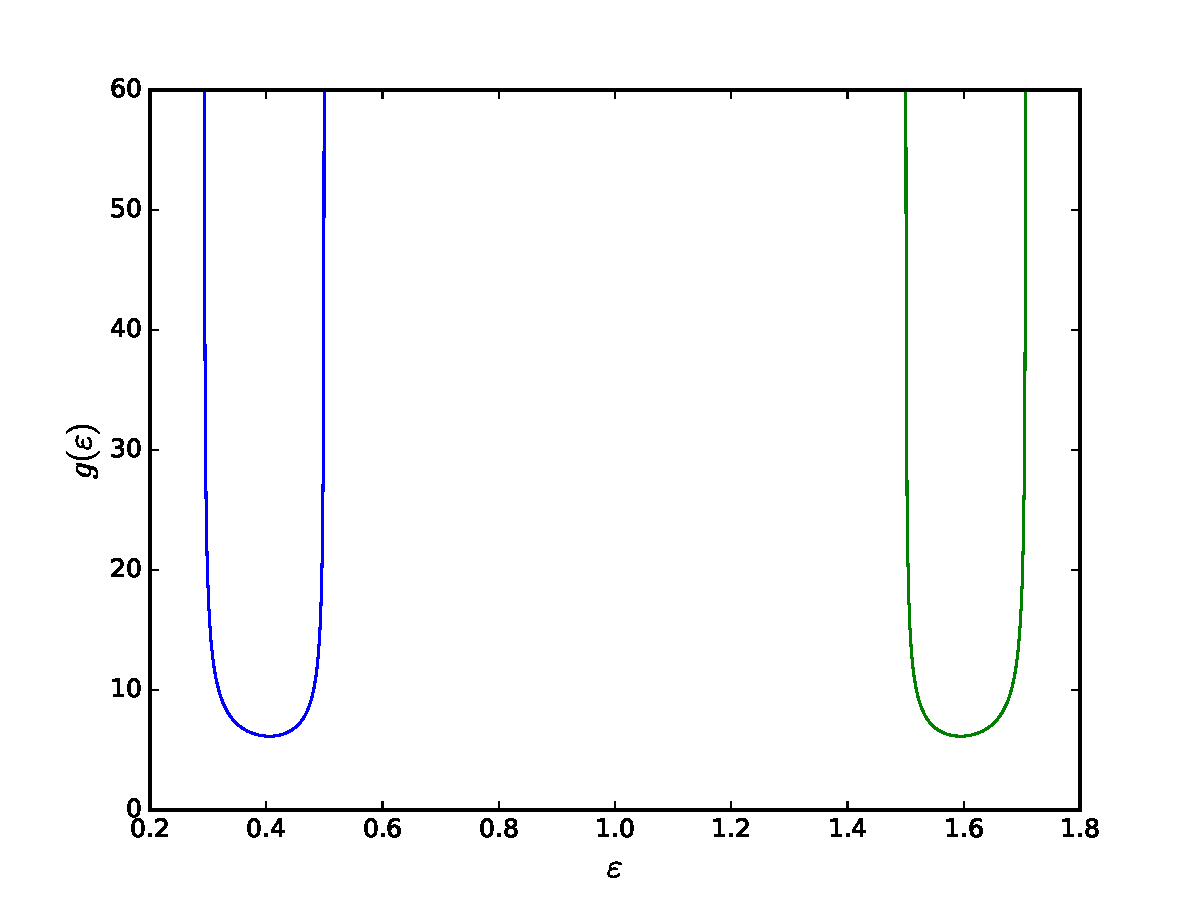
\includegraphics[width=0.7\linewidth]{pro_1_b.pdf}
              \caption{DOS.}
              \label{fig:pro1b}
          \end{figure}
    \item Suppose $\ket{\psi_{\bm{k}}} = c_1 \ket{d} + c_2 \ket{p}$. So the eigenvector satisfies
          the equation
          \begin{equation}
              (H_{\bm{k}} - \varepsilon I)\begin{pmatrix}
                  c_1 \\ c_2\\
              \end{pmatrix} = 0,
          \end{equation}
          solve this equation, we will derive $c_1$ and $c_2$, so
          \begin{equation}
              \begin{split}
                  \braket{d | \psi} & = c_1, \\
                  \braket{p | \psi} & = c_2.
              \end{split}
          \end{equation}
          So we have
          \begin{equation}
              \begin{split}
                  g_d(\varepsilon) & = g(\varepsilon) c_1^\ast c_1, \\
                  g_p(\varepsilon) & = g(\varepsilon) c_2^\ast c_2.
              \end{split}
          \end{equation}
          See Fig. \ref{fig:projected_DOS} for reference. Notice here
          d-state DOS plus p-state DOS equal to original DOS, to make it convenient
          to observe, I add $1$ to original DOS to distinguish d-state DOS plus p-state DOS.
          \begin{figure}[h]
              \centering
              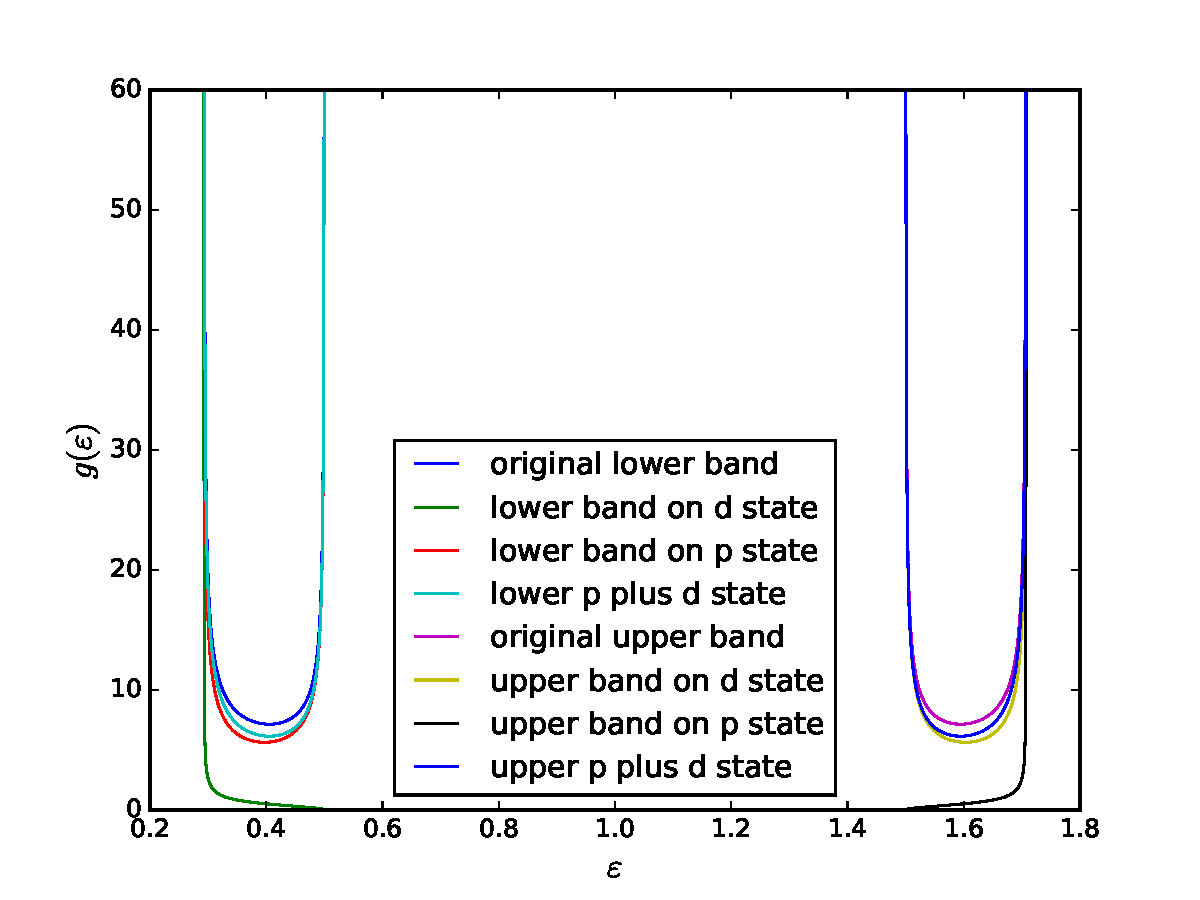
\includegraphics[width=0.7\linewidth]{pro_1_c}
              \caption{Projected DOS as well as original DOS.}
              \label{fig:projected_DOS}
          \end{figure}
    \item Assuming $\varepsilon_p=\frac{1}{2}$, Expand eigenvalue by assuming
          $t_{pd}$ is a very small number.
          The analytical eigenvalues are
          \begin{equation}
              \begin{split}
                  \varepsilon_1 & =\frac{1}{2}+\frac{1}{2}+\frac{1}{2}\sqrt{8 t^2 (\cos (k a)+1)+1}, \\
                  \varepsilon_2 & =\frac{1}{2}+\frac{1}{2}-\frac{1}{2}\sqrt{8 t^2 (\cos (k a)+1)+1}. \\
              \end{split}
          \end{equation}
          So by Taylor expansion, we derive
          \begin{equation}
              \begin{split}
                  \varepsilon_1 & \approx 2t^2 ( \cos (k a)+1)+\frac{3}{2}, \\
                  \varepsilon_2 & \approx -2t^2 ( \cos (k)+1)+ \frac{1}{2}. \\
              \end{split}
          \end{equation}
          Then plot them as Fig. \ref{fig:1-d}.
          \begin{figure}[h]
              \centering
              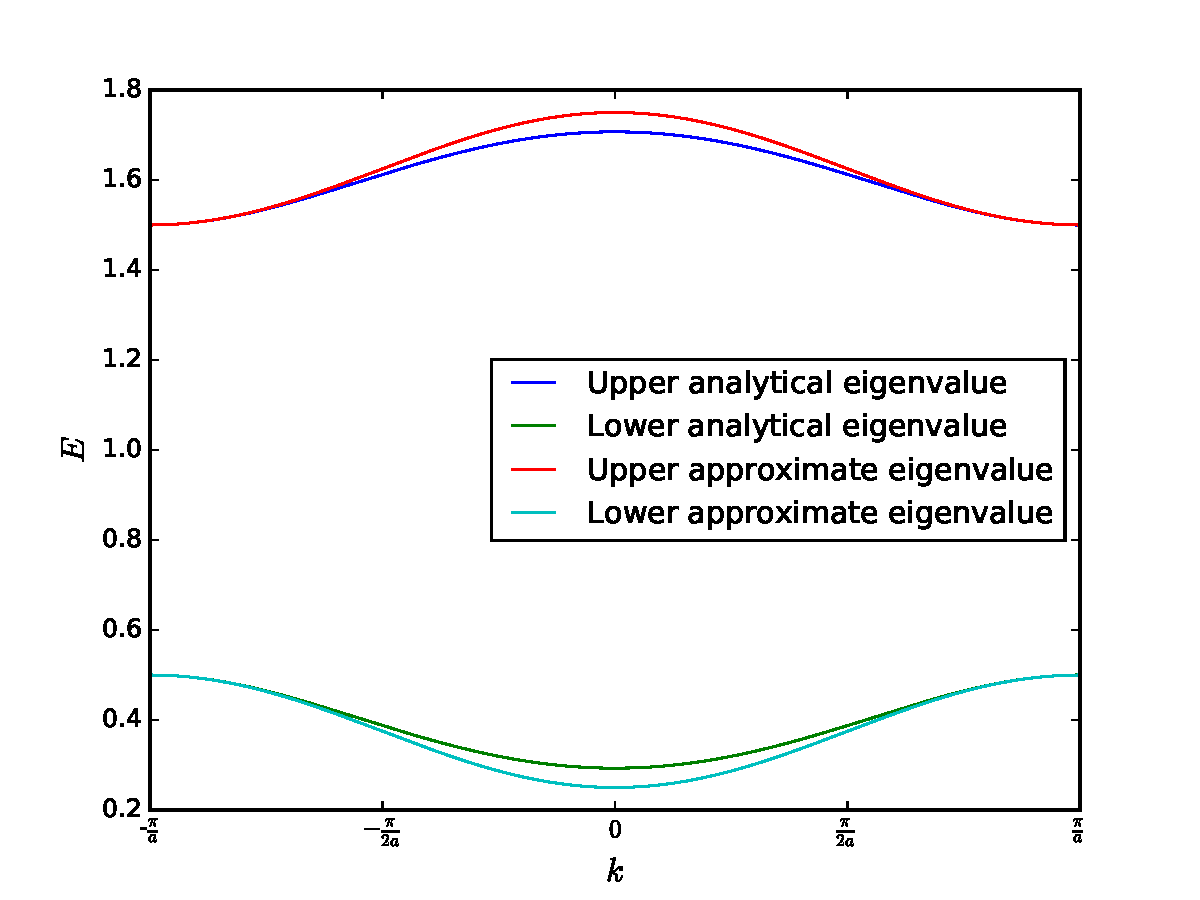
\includegraphics[width=0.7\linewidth]{pro_1_d}
              \caption{Analytical eigenvalue and approximate eigenvalue.}
              \label{fig:1-d}
          \end{figure}
    \item In the lower band, $2$ electrons were filled, and in upper bands,
          there fills $1$ electron. So $\varepsilon_F$ satisfy following equation
          \begin{equation}
              N(\varepsilon_F) = \frac{2}{\pi}\arccos(8(\varepsilon_F-1)^2-3) = 1,
          \end{equation}
          solve the equation, we derive $\varepsilon_F=\SI{1.61237}{\electronvolt}$.
\end{enumerate}

\section{Problem \RMN{2}}
\begin{enumerate}[(a)]
    \item Draw the graphene structure as Fig. \ref{fig:graphen}, with dashed line
          denoting a unit cell of graphene. Here the primitive vectors are $\bm{a}_1$ and $\bm{a}_2$,
          the primitive reciprocal vectors are $\bm{b}_1$ and $\bm{b}_2$, $a$ is
          the length of a hexagonal edge. If we set
          origin at the point where writes $\Gamma$, and use Cartesian coordinates,
          then
          \begin{align}
              \begin{cases}
                  \bm{a}_1 = (\frac{3a}{2}, - \frac{\sqrt{3a}}{2}), \\
                  \bm{a}_2 = (\frac{3a}{2}, \frac{\sqrt{3}a}{2}),   \\
              \end{cases} \\
              \begin{cases}
                  \bm{b}_1 = (\frac{2\pi}{3a}, - \frac{2\pi}{\sqrt{3}a}), \\
                  \bm{b}_2 = (\frac{2\pi}{3a}, \frac{2\pi}{\sqrt{3}a}).
              \end{cases}
          \end{align}
          \begin{figure}[h]
              \centering
              
\includegraphics[width=0.5\linewidth]{graphene.png}
              \caption{The honeycomb structure of graphene.}
              \label{fig:graphen}
          \end{figure}
          So in each cell, there are $2$ atomic orbitals, the red orbital and the green orbital.
          For green orbital, consider the eigenfunction
          of translation operator to be
          \begin{equation}
              \begin{split}
                  \psi(\bm{k}, \bm{r})
                   & = \frac{1}{\sqrt{1\times 3}} \sum_\nu \sum_{\bm{R}} \exp(i\bm{k}
                  \cdot \bm{R}) \phi_\nu(\bm{r}-\bm{R})                                      \\
                   & = \frac{1}{\sqrt{3}} \Big(\phi_{1}(\bm{r}) + \sum_{\bm{R}} \exp(i\bm{k}
                  \cdot \bm{R}) \phi_{2}(\bm{r}-\bm{R})\Big),
              \end{split}
          \end{equation}
          where $\phi_1(\bm{r})$ denotes green orbital itself, $\phi_2(\bm{r})$
          denotes $3$ nearest red orbitals.
          Similarly, for red orbital, the eigenfunction
          of translation operator is
          \begin{equation}
              \psi(\bm{k}', \bm{r})
              = \frac{1}{\sqrt{3}} \Big(\phi_{2}(\bm{r}) + \sum_{\bm{R}'} \exp(i\bm{k}'
              \cdot \bm{R}') \phi_{1}(\bm{r}-\bm{R}')\Big).
          \end{equation}
          So the Hamiltonian is
          \begin{equation}
              \begin{split}
                  H_{\bm{k}}
                   & = \sum_{\mu,\nu}\sum_{\bm{R}} \exp(i\bm{k}\cdot\bm{R})
                  \braket{\phi_\mu(\bm{r}) | H | \phi_\nu(\bm{r} - \bm{R})},
              \end{split}
          \end{equation}
          where
          \begin{equation}
              \begin{split}
                  \braket{\phi_1(\bm{r}) | H | \phi_1(\bm{r})}              = 0,                             \\
                  \braket{\phi_1(\bm{r}) | H | \phi_2(\bm{r}- (-a, 0))} =
                  \braket{\phi_1(\bm{r}) | H | \phi_2(\bm{r} - (\tfrac{1}{2}a, -\tfrac{\sqrt{3}}{2}a))} =
                  \braket{\phi_1(\bm{r}) | H | \phi_2(\bm{r} - (\tfrac{1}{2}a, \tfrac{\sqrt{3}}{2}a))} = t,  \\
                  \braket{\phi_2(\bm{r}) | H | \phi_1(\bm{r} - (a, 0))} =
                  \braket{\phi_2(\bm{r}) | H | \phi_1(\bm{r} - (-\tfrac{1}{2}a, \tfrac{\sqrt{3}}{2}a))} =
                  \braket{\phi_2(\bm{r}) | H | \phi_1(\bm{r} - (-\tfrac{1}{2}a, -\tfrac{\sqrt{3}}{2}a)} = t, \\
                  \braket{\phi_2(\bm{r}) | H | \phi_2(\bm{r})}              = 0.
              \end{split}
          \end{equation}
          Written as matrix form, it will be
          \begin{equation}
              H_{\bm{k}} =
              \begin{pmatrix}
                  0      & h \\
                  h^\ast & 0 \\
              \end{pmatrix},
          \end{equation}
          where $h = t\Big(e^{-i k_x a}
              + e^{i \Big(\tfrac{1}{2}k_x a - \tfrac{\sqrt{3}}{2}k_y a\Big)}
              + e^{i \Big(\tfrac{1}{2}k_x a + \tfrac{\sqrt{3}}{2}k_y a\Big)}\Big)$,
          and $h^\ast$ is its complex conjugate.
          So the analytical eigenvalues are
          \begin{equation}\label{eq:graphene_eig}
              \begin{split}
                  E_{\pm} & = \pm \sqrt{t^2 h^\ast h}                                                                                                    \\
                          & =\pm 2.5 \sqrt{4 \cos \Big(\frac{3 k_x a}{2}\Big) \cos \Big(\frac{\sqrt{3} k_y a}{2}\Big)+2 \cos \Big(\sqrt{3} k_y a\Big)+3}
              \end{split}
          \end{equation}
    \item The coordinates $(k_x, k_y)$ of $\Gamma$, $\mathrm{M}$ and $\mathrm{K}$ points
          are $(0, 0)$, $(\frac{2\pi}{3a}, 0)$,
          and $(\frac{2\pi}{3a}, \frac{2\pi}{3\sqrt{3}a})$, respectively.
          See Fig. \ref{fig:graphene:mini:subfig:b} for energy along the k-path.
          \begin{figure}[h]
              \subfigure[Density plot of graphene band structure.]{
                  \label{fig:graphene:mini:subfig:a}   %% label for first subfigure
                  \begin{minipage}[b]{0.5\textwidth}
                      \centering
                      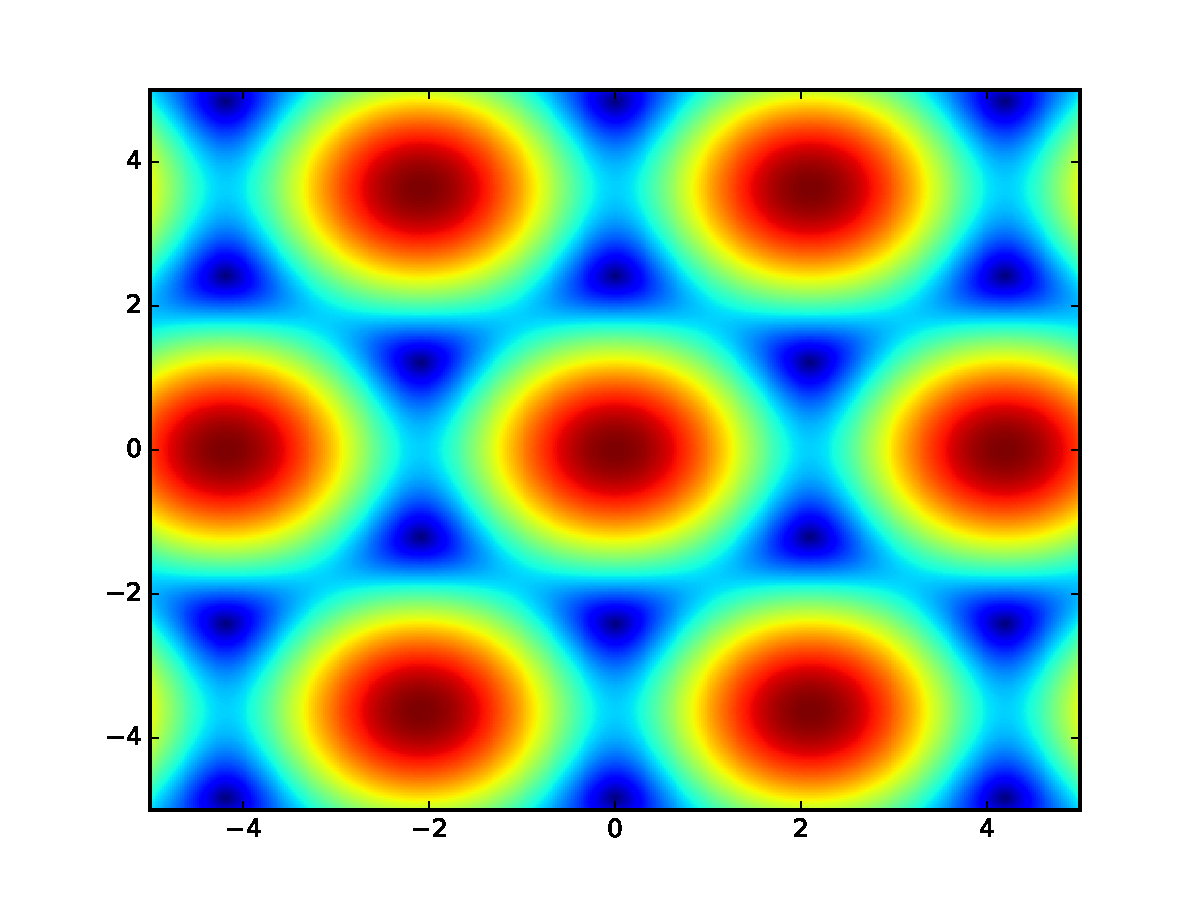
\includegraphics[width=\linewidth]{pro-2-b-1}
                  \end{minipage}}
              \hfill
              \subfigure[Energy along k-path.]{
                  \label{fig:graphene:mini:subfig:b}   %% label for second subfigure
                  \begin{minipage}[b]{0.5\textwidth}
                      \centering
                      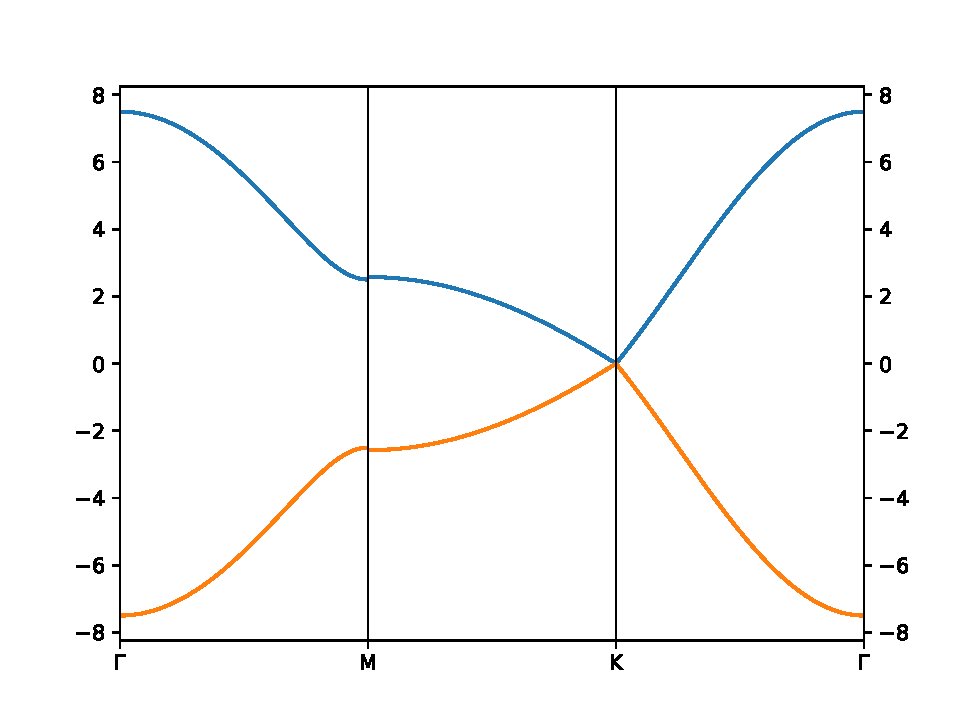
\includegraphics[width=\linewidth]{pro-2-b-2}
                  \end{minipage}}
              \caption{Some plots of graphene band structure.}
              \label{fig:along-k-path}   %% label for entire figure
          \end{figure}
    \item Because there are $2$ electrons per unit cell, assuming $N$ unit
          cells in the crystal, so there are $2N$ electrons in the crystal. Those
          electrons fully filled the lowest band in first BZ. So the Fermi energy
          is the maximum energy of the lowest band. From the figure we can see
          it is at $\mathrm{K}$ point, so the Fermi energy is \SI{0}{\electronvolt}.
    \item Let $k_x' = \frac{2\pi}{3a} + dk_x$, $k_y' = \frac{2\pi}{3\sqrt{3}a} + dk_y$, substitute into \eqref{eq:graphene_eig},
          and use approximation $\cos(x) \approx 1 - \frac{x^2}{2}$ and $\sqrt{1+x}\approx
              1+\frac{1}{2}x$, we derive
          \begin{equation}
              \begin{split}
                  \varepsilon & = \pm 2.5 \sqrt{4 \cos \Big(\frac{3 (\frac{2\pi}{3a}+dk_x) a}{2}\Big)
                  \cos \Big(\frac{\sqrt{3} (\frac{2\pi}{3\sqrt{3}a}+dk_y) a}{2}\Big)+2 \cos \Big(\sqrt{3} \Big(\frac{2\pi}{3\sqrt{3}a}+dk_y\Big) a\Big)+3} \\
                              & \approx \pm \frac{3ta}{2}\sqrt{dk_x^2 + dk_y^2}                                                                            \\
                              & = \pm \frac{3ta}{2} k.
              \end{split}
          \end{equation}
          So the dispersion relation is linear near the $\mathrm{K}$ point.
    \item We have
          \begin{equation}
              N(\varepsilon) = \frac{2}{V_{\text{FBZ}}}
              \int d\bm{k} \theta(\varepsilon - \varepsilon(\bm{k})),
          \end{equation}
          where $V_{\text{FBZ}} = \frac{8\pi^2}{3\sqrt{3}a^2}$ is the volume of the first BZ,
          and $\theta$ is Heaviside step function.
          \begin{figure}[h]
              \centering
              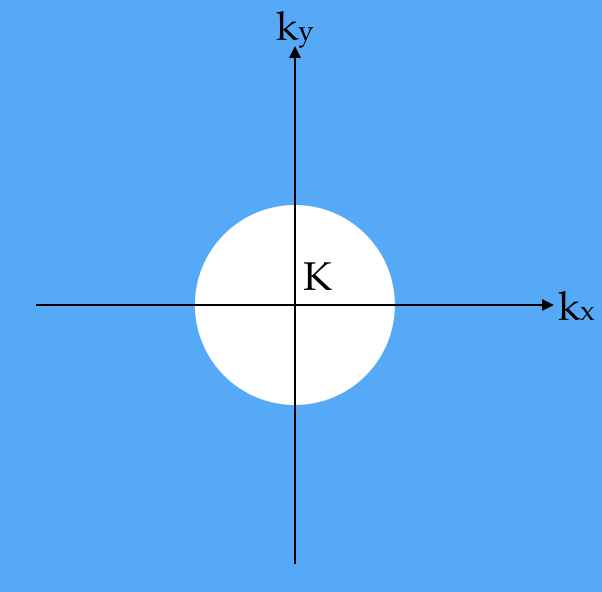
\includegraphics[width=0.3\linewidth]{2-e}
              \caption{Schemetic plot of filled band with $\mathrm{K}$ point as origin.}
              \label{fig:kx-ky}
          \end{figure}
          For a certain $\varepsilon$, only $\varepsilon(\bm{k}) < \varepsilon$ can
          be counted.
          Because in this question, the electrons fully filled the first band, and in the
          first band there are $2$ electrons. Thus, if we want to count the electrons
          within energy interval $\varepsilon < \varepsilon(\bm{k}) < \varepsilon_F$,
          we use
          \begin{equation}
              \begin{split}
                  N'(\varepsilon) & = \frac{2}{V_{\text{FBZ}}}
                  \int \theta(\varepsilon - \varepsilon(\bm{k})) d\bm{k}                       \\
                                  & = \frac{2}{V_{\text{FBZ}}}
                  \int_{\lvert \varepsilon(\bm{k}) \rvert < \lvert \varepsilon \rvert} d\bm{k} \\
                                  & = 2 - \frac{2}{V_{\text{FBZ}}}
                  \int_{\lvert \varepsilon \rvert \leq \lvert \varepsilon(\bm{k}) \rvert \leq \lvert \varepsilon_F\rvert}
                  d\bm{k}                                                                      \\
                                  & = 2 - \frac{2}{V_{\text{FBZ}}}
                  \int_{0 < k_x^2 + k_y^2 < k^2} dk_x dk_y                                     \\
                                  & = 2 - \frac{2}{V_{\text{FBZ}}}\pi k^2                      \\
                                  & = 2 - \frac{3 \sqrt{3} a^2 k^2}{4 \pi }.
              \end{split}
          \end{equation}
          See Fig. \ref{fig:kx-ky}, within the white circle $k_x^2 + k_y^2 < k^2$,
          those are the unfilled region whose energy is above $\varepsilon$.
          However, near the $\mathrm{K}$ point, as above,
          \begin{equation}
              k = \frac{2\varepsilon}{3 a t},
          \end{equation}
          so
          \begin{equation}
              N'(\varepsilon) = 2 - \frac{\varepsilon^2}{\sqrt{3}\pi t^2},
          \end{equation}
          So the DOS is the derivative of $N'(\varepsilon)$, written as
          \begin{equation}
              \begin{split}
                  g(\varepsilon) & = \frac{dN'(\varepsilon)}{d\varepsilon}      \\
                                 & = - \frac{2 \varepsilon}{\sqrt{3} \pi  t^2}.
              \end{split}
          \end{equation}
          Here $\varepsilon$ is below $\varepsilon_F$ (\SI{0}{\electronvolt}), so $g(\varepsilon)$ is
          still greater than $0$.
\end{enumerate}

\end{document}
